\section{Numerical Results}
\label{sec:experiments}

\subsection{Examples of running Simulated Annealing}

\begin{table}[h]
    \center
    \caption{Simulated Annealing with BR test to $\tau=10^{-7}$}
    \label{table:run_example}
    \footnotesize
    \setstretch{1.5}
    \begin{tabular}{c|cc|cc}
& $\vect{x}^\star$ & $f(\vect{x}^\star)$ & $\# f$ evals & $\# \nabla f$ evals \\
\hline
1 & ( 9.42478, 2.47500 ) & 0.39789 & 448 & 166 \\
2 & ( 9.42478, 2.47500 ) & 0.39789 & 607 & 224 \\
3 & ( 9.42478, 2.47500 ) & 0.39789 & 688 & 232 \\
4 & ( -3.14159, 12.27500 ) & 0.39789 & 567 & 167 \\
5 & ( -3.14159, 12.27500 ) & 0.39789 & 648 & 195 \\
6 & ( -3.14159, 12.27500 ) & 0.39789 & 568 & 199 \\
7 & ( 3.14159, 2.27500 ) & 0.39789 & 529 & 183 \\
8 & ( 3.14159, 2.27500 ) & 0.39789 & 486 & 172 \\
9 & ( 3.14159, 2.27500 ) & 0.39789 & 528 & 204 \\
10 & ( -3.14159, 12.27500 ) & 0.39789 & 527 & 190 \\
11 & ( 3.14159, 2.27500 ) & 0.39789 & 607 & 195 \\
12 & ( -3.14159, 12.27500 ) & 0.39789 & 568 & 201 \\
13 & ( -3.14159, 12.27500 ) & 0.39789 & 489 & 179 \\
14 & ( -3.14159, 12.27500 ) & 0.39789 & 608 & 203 \\
15 & ( 9.42478, 2.47500 ) & 0.39789 & 728 & 228 \\
16 & ( 3.14159, 2.27500 ) & 0.39789 & 528 & 179 \\
17 & ( 9.42478, 2.47500 ) & 0.39789 & 728 & 235 \\
18 & ( 3.14159, 2.27500 ) & 0.39789 & 567 & 201 \\
19 & ( 3.14159, 2.27500 ) & 0.39789 & 649 & 225 \\
20 & ( 3.14159, 2.27500 ) & 0.39789 & 767 & 244 \\
    \end{tabular}
    
    \vspace{10pt}

    \Cref{table:run_example}: note that all 3 global minima are found. The following parameters were used and serve as good
    default paramters: $L_0 = 20, \delta=1.1, \epsilon_s = 10^{-6}, \chi=0.9, \gamma=10^{-2}$ and
    $T=0.5$.
\end{table}

\begin{figure}
    \centering
    \caption{Average SA trajectories for BR}
    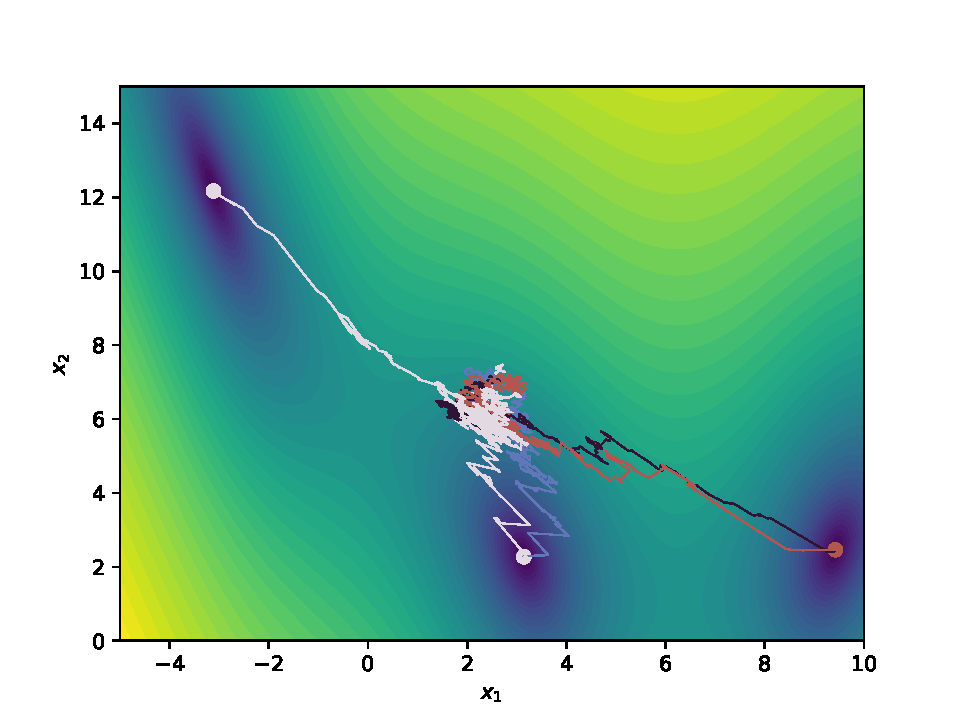
\includegraphics[scale=0.42]{figures/fig51-branin.pdf}
    \label{fig:5.1.1}
\end{figure}

\begin{figure}
    \centering
    \caption{Average SA trajectories for GP}
    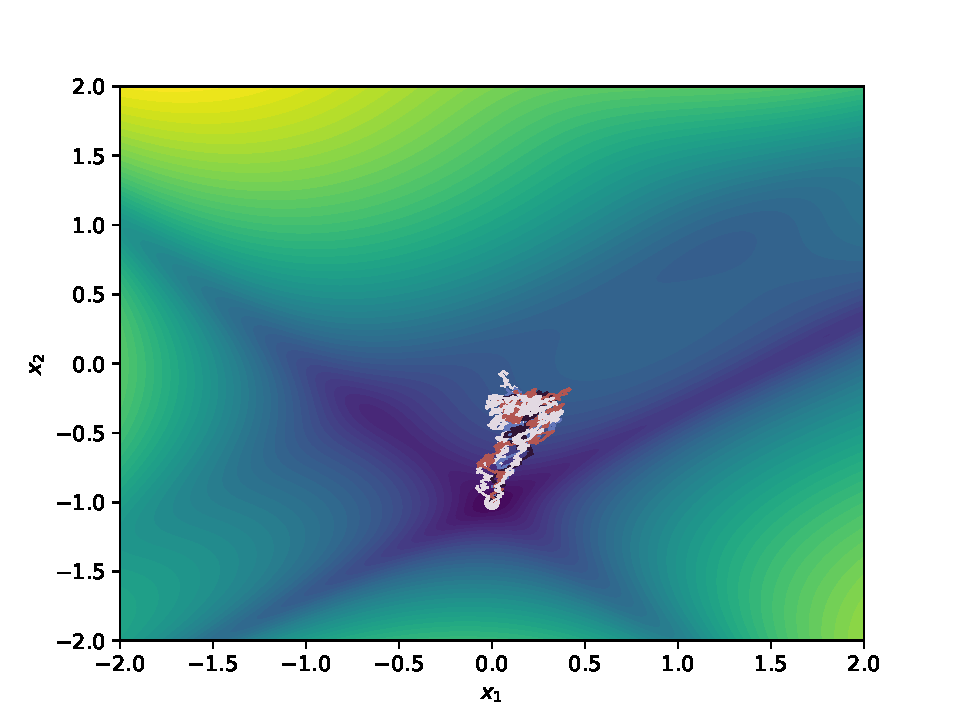
\includegraphics[scale=0.42]{figures/fig51-goldstein_price.pdf}
    \label{fig:5.1.2}
\end{figure}

\begin{table}
    \center
    \caption{Average number of runs required to solve problems}
    \label{table:run_numbers}
    \footnotesize
    \setstretch{1.5}
    \begin{tabular}{cc|cccc}
        & Problem & Avg. num runs & Solutions found & $\# f$ evals & $\# \nabla f$ evals \\
        \hline
1 & RB & 1.0 & 1 & 614.58 & 210.68 \\
1 & GP & 1.6 & 1 & 1072.38 & 385.96 \\
3 & BR & 5.18 & 3 & 3012.68 & 1041.06 \\
1 & H3 & 1.12 & 1 & 575.08 & 211.06 \\
1 & H6 & 1.58 & 1 & 737.7 & 284.1 \\
    \end{tabular}

\end{table}
    
\Cref{table:run_numbers} shows average required number of runs for the benchmark problems RB, GP, BR, H3, and H6, Simulated Annealing is run
repeatedly until all known global minima are found for the problem. A solution $\hat{\vect{x}}_i$ is considered the same
if $|\hat{\vect{x}}_i - \vect{x}^\star_j|_2 \leq \tau = 10^{-4}$.
This process is repeated $M=50$ times
and average number of runs, average function and Jacobian values are reported. In all cases, every global minimum
was found. Test problems BR and H6 show an average higher number of required runs per global minima. 

The following
Simulated Annealing parameters were used: $l_0=20, \delta=1.1, \epsilon_s=1e-4, \chi=0.9,
\gamma=10^{-2}$, and $t=0.5$.


\begin{table}
    \center
    \caption{Global and local minima found by Simulated Annealing}
    \label{table:minima}
    \footnotesize
    \setstretch{1.5}
    \begin{tabular}{rc|lr}
        Prob & Type & $\vect{x}^\star_i$ & $f(\vect{x}^\star_i)$ \\
        \hline
RB & g & ( 1.0, 1.0 ) & 0.0 \\
\hline
GP & g & ( -0.0, -1.0 ) & 3.0 \\
& l &( -0.6, -0.4 ) & 30.0 \\
& & ( 1.8, 0.2 ) & 84.0 \\
\hline
BR & g & ( -3.14159, 12.275 ) & 0.39789 \\
& & ( 3.14159, 2.275 ) & 0.39789 \\
& & ( 9.42478, 2.475 ) & 0.39789 \\
\hline
H3 & g & ( 0.11461, 0.55565, 0.85255 ) & -3.86278 \\
& l &( 0.10934, 0.86052, 0.56412 ) & -3.08976 \\
\hline
H6 & g & ( 0.20169, 0.15001, 0.47687, 0.27533, 0.31165, 0.6573 ) & -3.32237 \\
& l &( 0.40465, 0.88244, 0.8461, 0.57399, 0.13893, 0.0385 ) & -3.20316 \\
\end{tabular}
\end{table}


%\subsection{Exploring the hyper parameter space}

%Our implementation of Simulated Annealing has the following hyper parameters:

%\begin{itemize}
%    \item $L_0\in\Nat$ - the unit length which determines the length of the Markov chains
%    \item $\delta\in (1,\infty)$ - determines the rate at which the temperature parameter $c$ is decremented
%    \item $\epsilon_s\in\Real_+$ - the stopping parameter
%    \item $\chi \in (0,1)$ - initial acceptance parameter used to determine $c_0$
%    \item $\gamma \in (0, 1)$ - the smoothing parameter to filter out excess variance of $\overline{f_s}(c)$
%    \item $T$ - descent affinity, controls the likelihood of generating a new point along a descent
%    direction as opposed to uniform sampling
%\end{itemize}

%To better understand the role each of these parameters play in the performance of the simulated annealing algorithm,
%we performed Bayesian hyper parameter optimization using the Python black-box hyper parameter optimization framework
%\emph{Optuna}. We search the parameter space 
%$\vect{\Theta}=\begin{pmatrix} L_0 & \delta & \epsilon & \chi & \gamma & T\end{pmatrix}^T$.
%To measure the efficiency a chosen set of parameters, we define the objective function

%The number of Markov chains $n^{(i)}$, including required repeats, on the $i$-th run is given a $\nu$-weighted penalty:

%$$
%\nu n^{(i)} d L_0
%$$

%\begin{equation}
%    g_1(\vect{\Omega}) = \frac{1}{k}\left( \sum_{i=1}^k f(\hat{\vect{x}}_i) + \nu n^{(i)} d L_0\right)
%\end{equation}

%where for each $\vect{\Omega}$, simulated annealing is repeated $k$ times, and $\hat{\vect{x}}^{(i)}$ is the solution of
%the $i$-th run. $g_1$ is simply the average minimum of the solutions of $k$ with a penalty term.

%\begin{equation}
%    g_2(\vect{\Omega}) = \frac{1}{k}\sum_{i=1}^k \min_j \left\lbrace 
%    \left|\left| \vect{\hat{x}}^{(i)} - \vect{x}^\star_j \right|\right|_2
%    \right\rbrace
%\end{equation}

%If the set of global minimizers of $f$ is $\left\lbrace \vect{x}^\star_j \right\rbrace_{j=1}^J$, then 
%$g_2$ is the average $L_2$ distance to the nearest global minimizer $\vect{x}^\star_j$ of $f$ from the solution
%$\vect{\hat{x}}^{(i)}$ found in the $i$-th run.
